\begin{figure}[h]
 \centering
 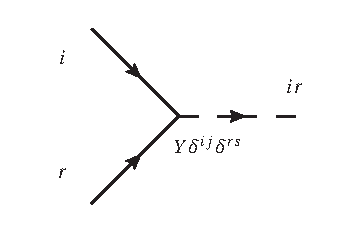
\includegraphics{abschnitte/QCDxdQCD/fig/Yukawa.eps}
 \caption{Möglicher Yukawa-Vertex in $SU(\Nc)\times SU(\Nd)$. Die Pfeile 
 zeigen dabei die \QCDxdQCD Ladungserhaltung an.}
 \label{fig:QCDxdQCD:Yukawa_Majorana}
\end{figure}
